\documentclass[parskip=full]{scrartcl}
\usepackage[T1]{fontenc}
\usepackage[utf8]{inputenc}
\usepackage[german]{babel}
\usepackage{hyperref}
\usepackage{float}
\hypersetup{
pdftitle={PSE: Blockchain-basiertes E-Voting - Entwurfsdokument},%
,%
}
\usepackage{graphicx}
\usepackage{csquotes}
\usepackage[nonumberlist]{glossaries}
\usepackage{enumitem}
\usepackage{xcolor}
\usepackage{lscape}

\title{PSE: Blockchain-basiertes E-Voting}

\begin{document}
	\clearpage
	\maketitle
	\pagenumbering{gobble}
	\newpage
	
	\tableofcontents
	\newpage
	\pagenumbering{arabic}
	\section{Einleitung}
	\section{Klassenbeschreibungen}
	\subsection{ViewToModelIF}
	Das ViewToModelIF bietet der View ein Interface um auf die Datenhaltung zuzugreifen.
	Es werden Methoden bereitgestellt, die es ermöglichen allgemeine Daten zur Wahl abzufragen.
	Die hiervon ausgehenden konkreten Interfaces SupervisorViewToModelIF und VoterViewToModelIF stellen zusätzlich Methoden zur Verfügung. Diese fragen Daten ab, die lediglich für den Wahlleiter oder respektive nur für den Wähler relevant sind.
	Die Methode setElectionEndListener dient dem Festlegen eines ActionListeners für das Wahlende beim initialen starten des Programms.
	
	\subsection{ControlToModelIF}
	Das ControlToModelIF bietet der Control ein Interface um auf die Datenhaltung zuzugreifen.
	Es werden Methoden bereitgestellt, die es ermöglichen die Daten auf der Datenhaltung zu manipulieren und entsprechende Zugriffe auf das Blockchain Netzwerk auszuführen.
	Die hiervon ausgehenden konkreten Interfaces VoterControlToModelIF und SupervisorControlToModelIF stellen zusätzlich Methoden zur Verfügung. Diese ermöglichen Netzwerkzugriffe und Datenmanipulation, die lediglich für den Wahlleiter oder respektive nur für den Wähler relevant oder erlaubt sind.
	
	\section{Sequenzdiagramme}
	\begin{figure}[H]
		\centering
		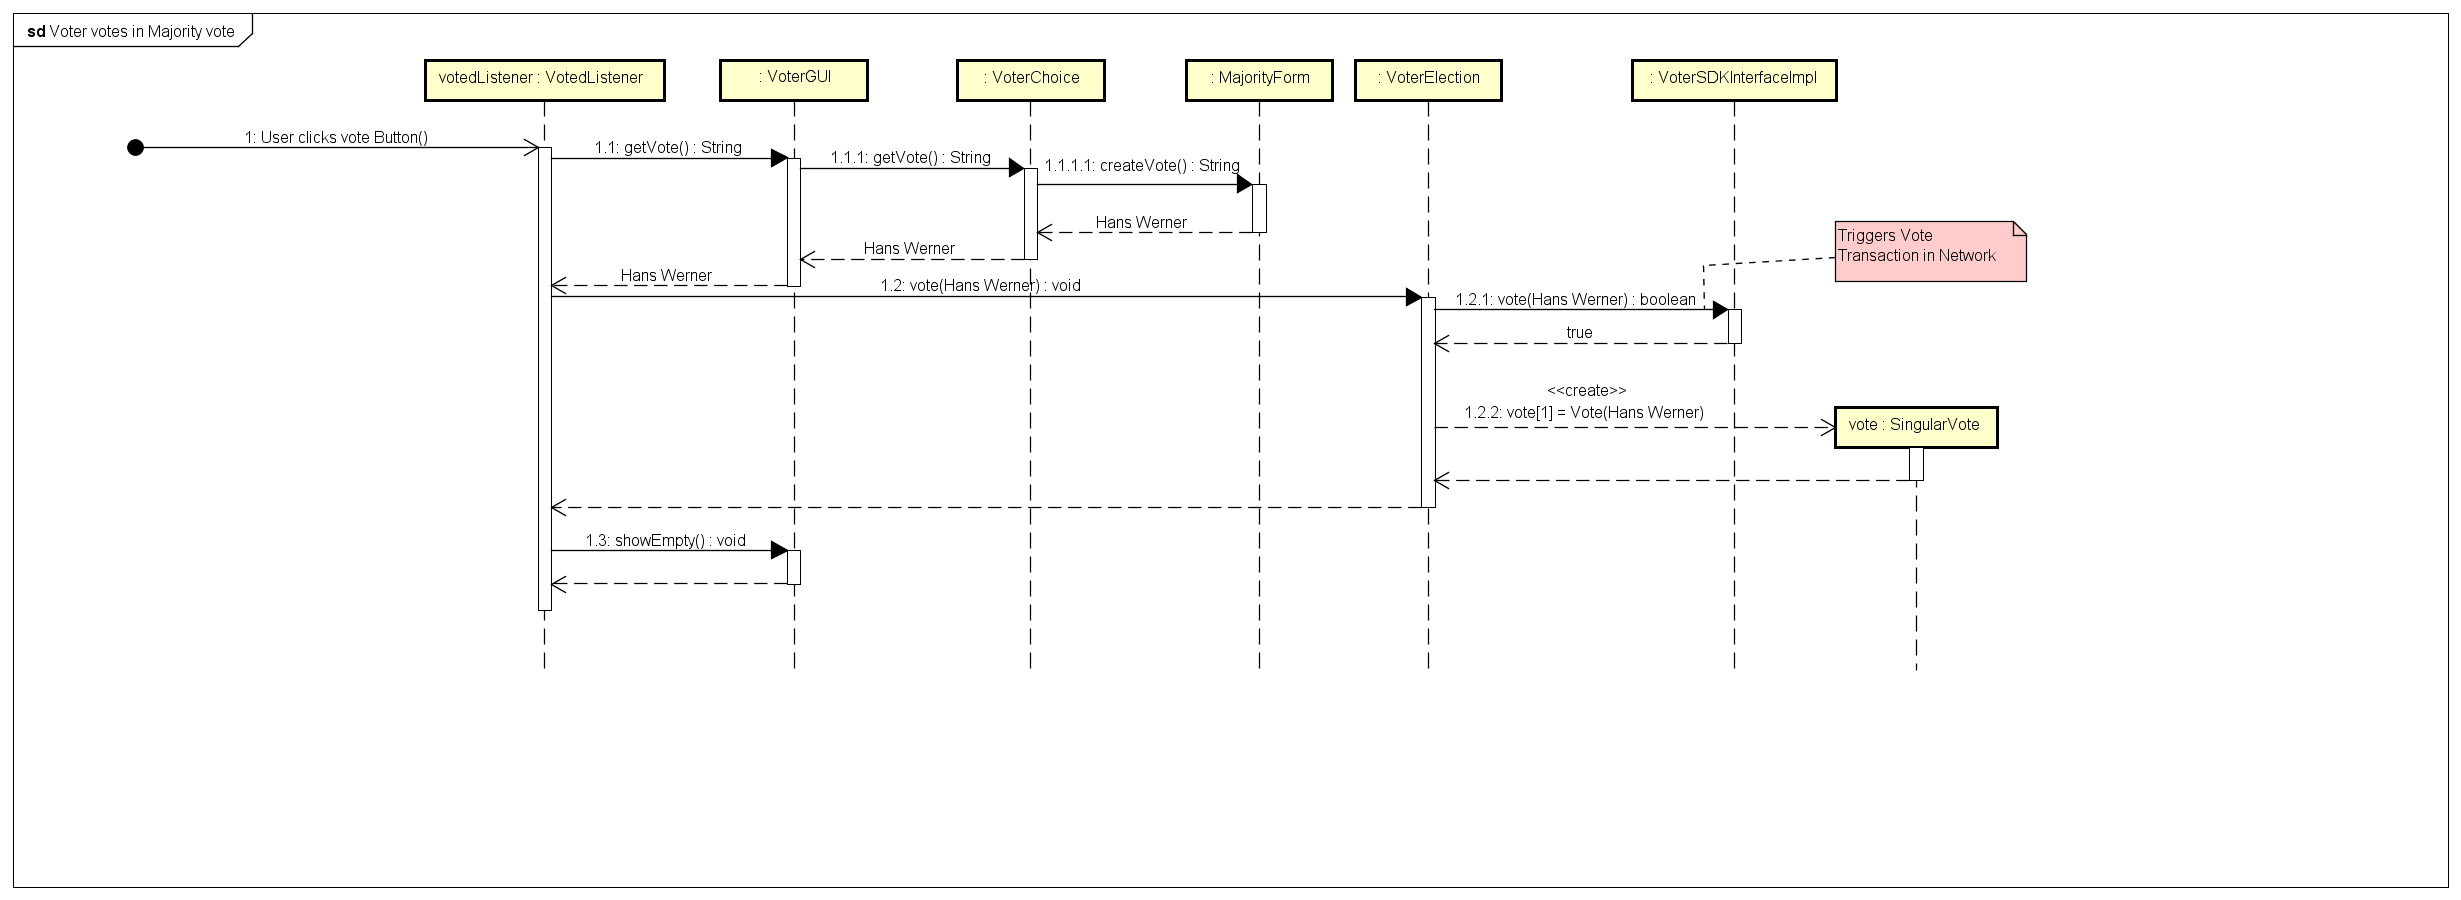
\includegraphics[scale=0.25]{graphics/simpleVote.png}
		\caption{Ablauf einer Stimmabgabe aus Sicht des Wählers}
	\end{figure}
	
	\newpage
	
\end{document}